\documentclass[12pt,a4paper]{report}

% Reference to title and author
\usepackage{titling}

% Fonts
\usepackage{titlesec}
\usepackage{helvet}
\usepackage{mathptmx}

% Chapter titles
\titleformat{\chapter}
{\Huge\bfseries\normalfont\sffamily}{\thechapter}{1em}{}
\titlespacing*{\chapter}{0pt}{3ex}{2.3ex plus .2ex}
\usepackage[english]{babel}
\usepackage[utf8]{inputenc}
\usepackage[T1]{fontenc}
\usepackage{lmodern}

% Hyperlinks
\usepackage[hidelinks]{hyperref}

% Appendices
\usepackage[toc,page]{appendix}
\usepackage[backend=bibtex8,style=ieee]{biblatex}
\bibliography{bibliography.bib}

% Images
\usepackage{graphicx}

% Framed boxes
\usepackage{framed}

% Page margins
\usepackage{geometry}
\geometry{margin=0.9in}

% Floats
\usepackage{float}

% Listings
\usepackage{dirtree}
\usepackage{listings}
\usepackage{color}

\definecolor{dkgreen}{rgb}{0,0.6,0}
\definecolor{gray}{rgb}{0.5,0.5,0.5}
\definecolor{mauve}{rgb}{0.58,0,0.82}

\lstset{frame=tb,
language=Python,
aboveskip=3mm,
belowskip=3mm,
showstringspaces=false,
columns=flexible,
basicstyle={\scriptsize\ttfamily},
numbers=none,
numberstyle=\tiny\color{gray},
keywordstyle=\color{blue},
commentstyle=\color{dkgreen},
stringstyle=\color{mauve},
breaklines=true,
postbreak=\mbox{\textcolor{red}{$\hookrightarrow$}\space},
breakatwhitespace=true,
tabsize=2,
frame=single
}

\title{Danger-Zone: A comparative study of mixed-traffic scenarios using collective intelligence simulation}
\author{
Georgios Andreadis, Jackson Matlak,\\
Heather Taylor, Tanisha Servet
}
\date{\today}

\setcounter{tocdepth}{1}


\begin{document}

    \begin{titlepage}
        \centering

        
\includegraphics[width=1.5in]{images/vu-logo.png}\par
        \vspace{1cm}
        {\scshape\Large Collective Intelligence\par}
        \vspace{1.5cm}

        {\Huge\bfseries\normalfont\sffamily \thetitle \par}
        \par\vspace{1cm}
        {\Large\itshape \theauthor \par}
        \vspace{1.5cm}

        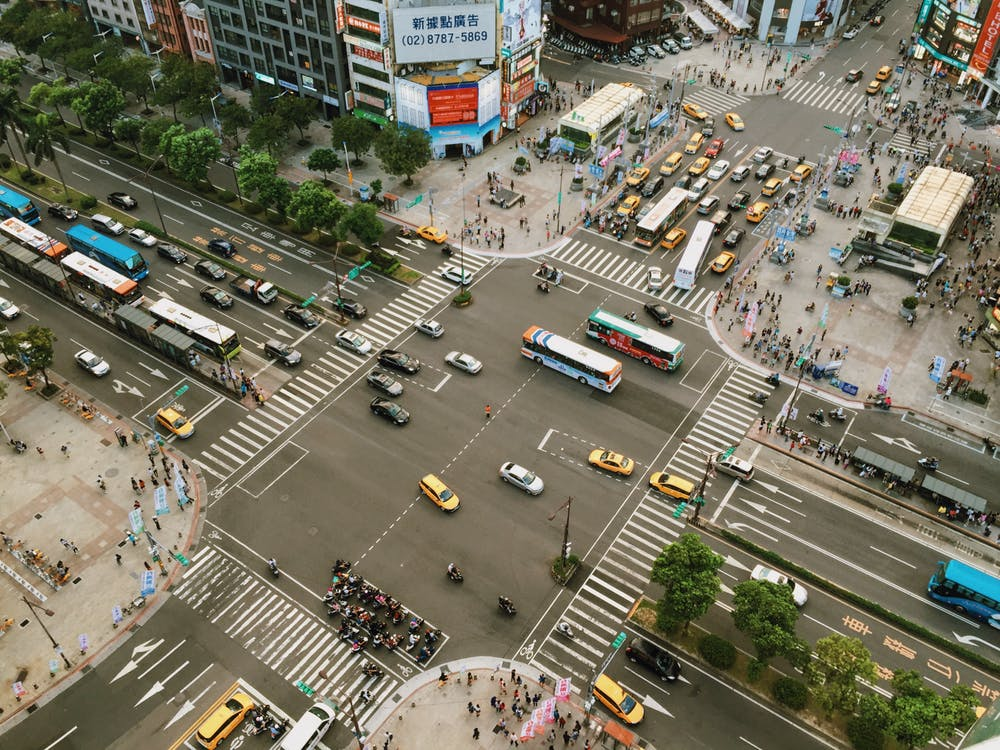
\includegraphics[width=15cm]{images/junction.jpeg}\par

        \vfill

        {\large \thedate \par}
    \end{titlepage}

    \begin{abstract}
    The rise of motorised travel has revolutionised how roads are used, and this can make travel challenging for pedestrians. One particular challenge has been the use of shared spaces -- areas where pedestrians and other vehicles utilise the road together, such as pedestrian crossings. This type of urban traffic layout has seen a recent surge in popularity, with multiple municipalities opting to implement it in highly frequented traffic locations. These layouts are often claimed to increase efficiency and decrease the risk of accidents, but existing traffic models have failed to analyse their full consequences. This paper proposes a new model, called `Danger Zone', which simulates some basic modes of transportation using an approach based on both cellular automata and agent system models to simulate what happens when pedestrians and other entities, such as cars, share spaces on the road. From this, the effects of shared spaces on traffic flow are observed and analysed, allowing an evaluation of slower designs and more accident-prone areas.
\end{abstract}

    \tableofcontents
    \chapter{Introduction} \label{chap:introduction}

\TODO{Write introduction chapter}

    \chapter{Related Work} \label{chap:related}

\TODO{Write related work chapter}
\cite{andreadis2017}
    \chapter{Algorithm Description} \label{chap:algorithm}

\TODO{Write algorithm chapter}

    \chapter{Experimental Setup} \label{chap:setup}

Our core set of experiments consists of two maps, both having two sidewalks and a two-lane road in the center. Pedestrian spawn points are on both ends of both sidewalks. To test our hypothesis, two modified versions of this map were made. The first has a small crosswalk area in the middle of the road, representing a traditional traffic situation in which pedestrians need to cross the road at a bottleneck to continue their journey. Map 2 has a significantly wider crosswalk area, representing a shared-space model for traffic. Both maps are defined in .dzone files, and can be seen in a folder on our GitHub repository\footnote{\url{https://github.com/gandreadis/danger-zone/tree/master/maps}}.

Command-line arguments are included in order to automate the running of multiple simulations, as well as set the number of ticks each will run for, and set the spawn delays for both cars and pedestrians.  Each of these were set and run for both maps, and a command line script running the entire set of parameter combinations tested can be found in the repository\footnote{\url{https://github.com/gandreadis/danger-zone/blob/master/experiment_scripts/straight_crosswalk_experiment.cmd}}.

\section{Number of Ticks}
The simulation is tick-based, meaning that time is discretized into distinct intervals, and progress is evaluated at each of these. Inherent to any time-based simulation is the need to restrict its duration, under a certain exit criterion. In this series of experiments, the exit criterion was chosen to be 1000 ticks. Our initial explorations of parameter combinations indicated that this would strike a balance between conserving computation time and allowing more data and emergent behaviours to be produced.

\section{Pedestrian and Car Spawn Delays}
Agents are spawned periodically as a simulation runs, and as such these periods (i.e. the number of ticks between two spawns of a certain type) can be adjusted by command-line arguments in order to simulate different types of traffic load. Two series of runs were performed on each map: One with a fixed car spawn delay and increasing pedestrian spawn delay and one that fixed the pedestrian delay and increased the spawn delay (in order to only vary one parameter at a time). The exact values and combinations can be found in the experiment script.

\section{Number of Repeated Iterations}
Due to the non-deterministic nature of the randomised spawns, different simulation runs with the same parameters could lead to different results. To ascertain that the results did not rely on unrepresentative data, each combination of the above 3 parameters was repeated 10 times.

    \chapter{Results} \label{chap:results}

The experiments previously outlined produced a series of CSV files, which were aggregated and evaluated into one list of findings. In general, this result data exhibits a higher throughput for both pedestrians and cars in the larger crosswalk map compared to the smaller crosswalk map. Figure \ref{fig:plot-pedestrian-throughput} and \ref{fig:plot-car-throughput} plot pedestrian and car throughput (respectively) against varying spawn delays. These varying delays indicate different levels of load on the layout, where higher delay translates to lower load. Each point on the charts represents the average of ten repetitions in that configuration, to eliminate non-deterministic factors.

\begin{figure}[h]
    \centering
    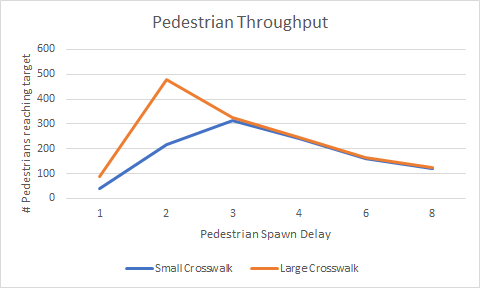
\includegraphics[width=4.2in]{images/plot-pedestrian-throughput.png}
    \caption{Plot of pedestrian throughput against pedestrian spawn delay, for both map layouts (car spawn delay is fixed at 5).}
    \label{fig:plot-pedestrian-throughput}
\end{figure}

\begin{figure}[h]
    \centering
    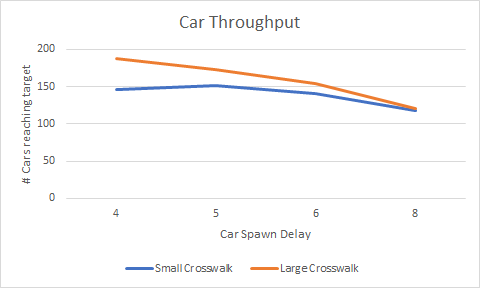
\includegraphics[width=4.2in]{images/plot-car-throughput.png}
    \caption{Plot of car throughput against car spawn delay, for both map layouts (pedestrian spawn delay is fixed at 5).}
    \label{fig:plot-car-throughput}
\end{figure}

Figure \ref{fig:plot-pedestrian-throughput} shows pedestrian throughput over pedestrian spawn delays. At low spawn delay (1-2), the simulation quickly becomes crowded, and the larger crosswalk has significantly higher throughput. At higher delays (3+), congestion ceases to be an issue and this difference becomes negligible. Figure \ref{fig:plot-car-throughput}, on the other hand, shows a more consistent decline of car throughput over car spawn delay. The car throughput of the large crosswalk layout remains consistently greater than the car throughput of the small crosswalk. However, this difference decreases at longer car spawn delays, and the margin of performance between the two maps also becomes negligible.

Both of the central results shown in Figure \ref{fig:plot-pedestrian-throughput} and \ref{fig:plot-car-throughput} look at the average throughputs over iterations. To make certain that the average values were representative of their series, the variance of each series was also calculated. This variance decreased with decreasing traffic density, but stayed low throughout. Figures \ref{fig:plot-pedestrian-variance} and \ref{fig:plot-car-variance} show this effect for pedestrians and cars, respectively.

We also recorded the number of failed spawn attempts for each run. However, as this data is complementary to the throughput data, the one can be derived from the other (given the total number of agents of that type spawned). It thus provides little additional information, and will not be discussed further in this report.

\begin{figure}[h]
    \centering
    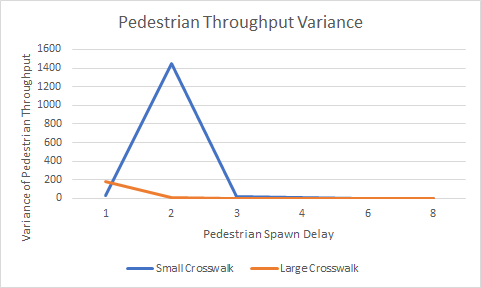
\includegraphics[width=4.2in]{images/plot-pedestrian-variance.png}
    \caption{Plot of pedestrian throughput variance against pedestrian spawn delay, for both map layouts (car spawn delay is fixed at 5).}
    \label{fig:plot-pedestrian-variance}
\end{figure}

\begin{figure}[h]
    \centering
    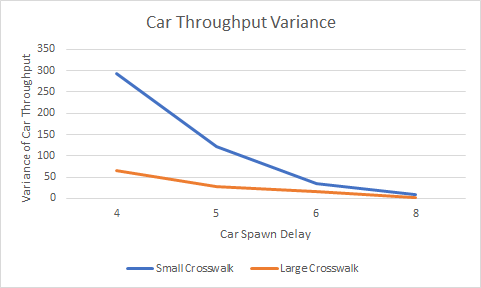
\includegraphics[width=4.2in]{images/plot-car-variance.png}
    \caption{Plot of car throughput variance against car spawn delay, for both map layouts (pedestrian spawn delay is fixed at 5).}
    \label{fig:plot-car-variance}
\end{figure}
    \chapter{Analysis} \label{chap:analysis}

The purpose of these experiments was to investigate which traffic layout benefits traffic participants most. From the data shown above, it is clear that throughput in the large crosswalk scenario is much more stable than in the small crosswalk scenario, both across runs and agent types. This can be seen in its overall lower and more monotonic variance. While this in itself does not yield conclusions on performance, it indicates that those travelling across this scenario can rely on a more predictable amount of time that they will need to get across.

The average throughput indicates another metric in which the large crosswalk surpasses the small crosswalk: For both pedestrians and cars, the time an agent requires to reach their target is reduced in the large crosswalk setting. This speaks in favour of the shared-space (large crosswalk) model, as its efficiency seems higher than its counterpart (small crosswalk).

In general, although the large crosswalk scenario does seem to perform better and more predictably, it must be noted that these differences only play a role in busy situations. As traffic load reduces, the differences become almost negligible. This indicates that these findings are likely to only be relevant for traffic sites that will be frequented by many participants simultaneously, and less so for less busy urban locations.

However, as with any computer model, there are several threats to the validity of these conclusions. This simulator has not been validated against real-world scenarios, due to us not having access to the kind of real-world measurement traces needed to compare our findings with realistic measurements of throughput. Only relying on visual verification and programmatic assertions does not guarantee that the simulation results are realistic. The simplicity of our model is another concern brought up by only using simulations. A model typically needs to simplify some aspects of a problem in order to be computable, ours is no different. We did not take into account social interactions such as eye contact or differing characteristics of participants. The simulation also assumes uniform speed across all cars, and instantaneous acceleration and breaking, which is also why collisions or near-miss scenarios are not simulated in this model. Although we believe all these parameters to be less crucial to the simulation than what is already in the model, it is difficult to predict what their influence would have been on the results that were obtained.


    \chapter{Discussion} \label{chap:discussion}

If nothing else, this project made us realise the complexity of modeling real-life traffic scenarios. We set out to compare different traffic layouts from the viewpoint of efficiency (throughput), and to this aim two different approaches were attempted. The first approach, consisting of free-moving agents, falls short of being able to accurately model complex map layout navigations. The second approach, which discretized the map field and used CA-like rules for decision making, comes closer to our goal of comparative traffic layout evaluation. It is able to measure throughput in simple traffic scenarios, and can be used to compare map layouts on their efficiency. However, it fails to model collisions, preventing any measurement of the safety of layouts.

Our initial goal was ambitious, as we discovered during design and development. A system without discrete steps models the world more accurately, but is significantly more difficult to design. We faced this when trying to give the free agents in our first design some type of pathfinding ability. On the other hand, the discrete steps system we selected was easier to design and implement, but it also resembled the real world less. On top of this fundamental dilemma came various difficulties, from diverging levels of Python programming knowledge within the team to a general lack of time due to various circumstances and absences.

In the end, we were able to tentatively show superiority of a shared-space model over a traditional model. This is, however, just the beginning. There is still plenty of area to explore in this field, as evidenced by the large body of existing work in this domain. Most importantly perhaps in our case would be the addition of bicycle agents: Their agility and position in traffic makes them a unique aspect, and leaves many questions open about how they influence traffic patterns. After having added cyclists, more complex scenarios could be tested. Although the tested scenarios exist in real life, they are limited in scope and complexity, and have a great deal of possible expansion. More research could also go into the social interactions that take place in a traffic situation. Possible interactions that the model could benefit from would be visual contact (deciding who takes precedence) or use of sound signals (bells or horns on bikes or cars).



    \begin{appendices}
        \chapter{References}
        \printbibliography[heading=none]
        \input{chapters/listing.tex}
    \end{appendices}

\end{document}
